\documentclass[12pt,a4paper]{article}
\usepackage{ctex}
\usepackage{amsmath,amscd,amsbsy,amssymb,latexsym,url,bm,amsthm}
\usepackage{epsfig,graphicx,subfigure}
\usepackage{enumitem,balance}
\usepackage{wrapfig}
\usepackage{mathrsfs, euscript}
\usepackage[usenames]{xcolor}
\usepackage{hyperref}
\usepackage[vlined,ruled,commentsnumbered,linesnumbered]{algorithm2e}
\usepackage{float}
\usepackage{array}
\usepackage{diagbox}
\usepackage{color}
\usepackage{indentfirst}
\usepackage{fancyhdr}
\usepackage{gensymb}
\usepackage{geometry}
\usepackage{setspace}
\usepackage{aurical}
\usepackage{times}
\usepackage{caption}
\usepackage{fontspec}
\usepackage{booktabs}
\setmainfont{Times New Roman}

\newtheorem{theorem}{Theorem}[section]
\newtheorem{lemma}[theorem]{Lemma}
\newtheorem{proposition}[theorem]{Proposition}
\newtheorem{corollary}[theorem]{Corollary}
\newtheorem{exercise}{Exercise}[section]
\newtheorem*{solution}{Solution}
\theoremstyle{definition}


\renewcommand{\thefootnote}{\fnsymbol{footnote}}

\newcommand{\postscript}[2]
 {\setlength{\epsfxsize}{#2\hsize}
  \centerline{\epsfbox{#1}}}

\renewcommand{\baselinestretch}{1.0}

\setlength{\oddsidemargin}{-0.365in}
\setlength{\evensidemargin}{-0.365in}
\setlength{\topmargin}{-0.3in}
\setlength{\headheight}{0in}
\setlength{\headsep}{0in}
\setlength{\textheight}{10.1in}
\setlength{\textwidth}{7in}
\makeatletter \renewenvironment{proof}[1][Proof] {\par\pushQED{\qed}\normalfont\topsep6\p@\@plus6\p@\relax\trivlist\item[\hskip\labelsep\bfseries#1\@addpunct{.}]\ignorespaces}{\popQED\endtrivlist\@endpefalse} \makeatother
\makeatletter
\renewenvironment{solution}[1][Solution] {\par\pushQED{\qed}\normalfont\topsep6\p@\@plus6\p@\relax\trivlist\item[\hskip\labelsep\bfseries#1\@addpunct{.}]\ignorespaces}{\popQED\endtrivlist\@endpefalse} \makeatother



\begin{document}
\noindent
%==========================================================
\noindent\framebox[\linewidth]{\shortstack[c]{
\Large{\textbf{Report on}}\vspace{1mm}\\ 
\Large{\emph{Visualization and exploration of Adult Dataset}}\vspace{1mm}\\
CS245, Data Science Foundation, Chaojun Lu, Autumn 2017 \vspace{1mm} \\
叶泽林 515030910468}}
\vspace{-1.5\baselineskip}

\renewcommand{\figurename}{Figure}
\section{Introduction} % or Problem Description ?

Currently, data science is becoming ubiquitous in our society and showing its essentiality in many domains (e.g. medical industry~\cite{medical1, medical2}, finance~\cite{finance}, social media~\cite{media1, media2}). With the rapid evolution and wide applications of data science, a series of efficient packages have been constantly developed~\cite{numpy, pandas, matplotlib, sklearn}. Utilizing these packages skillfully is of great importance nowadays. In this project, I tend to conduct an exploration over the \textit{Adult} dataset and visualize the results with some of these packages.

\vspace{-1\baselineskip}
\section{Approaches}

The \textit{Adult} dataset is in the format of .CSV with 16281 lines, each line contains some basic information (age, job, gender and etc) of an adults. I explore and extract the information hidden in the data with the following steps:
\begin{enumerate}
\item Read the data with \textit{pandas}~\cite{pandas} and reconstruct it as \textit{DataFrame} type.

\item Select a target attribute (e.g. work time per week) to conduct analysis.

\item Select two attributes to explore the relation between them.

\item Visualize all analysis results with \textit{matplotlib}~\cite{matplotlib} and \textit{pandas}.
\end{enumerate}


\section{Experiments}

\subsection{Experiments Setup}

Since the data is organized as .CSV format, it is easy to be recogbnized by \textit{pandas}. I first construct the dataset as a \textit{DataFrame} with 16281 lines and 15 columns, each line denotes the information of an adult while each column represents an attribute.

\subsection{The Distribution of Single Attribute}

Basically, it is of great importance to get the distribution of some attributes in the data. I hence explore some of them and visualize the results with different figure types.

\begin{enumerate}
\item The distribution of educational level in the dataset is shown in fig. \ref{fig::education_level}.

The result shows the educational background of many adults are high school or college, occupying more than half of the proportion. Only a few people owns bad educational background(e.g. preschool).

\item The distribution of family relations can refer to fig. \ref{fig::family}.

The result indicates more than half of the adults have set up a family, while there still exist many adults remain unmarried or not in family.

\item The weekly working time distribution can be found in fig. \ref{fig::work_time}.

This Kernel Density Estimation(KDE) figure shows that most adults work 40 hours per week, and a few people also work more than 60 hours per week. I will conduct some deep explorations in Sec. \ref{sec::salary_vs_edu}.

\end{enumerate}

\begin{figure}[htbp]
	\centering
	\subfigure[Education Distribution]{
		\label{fig::education_level}
	    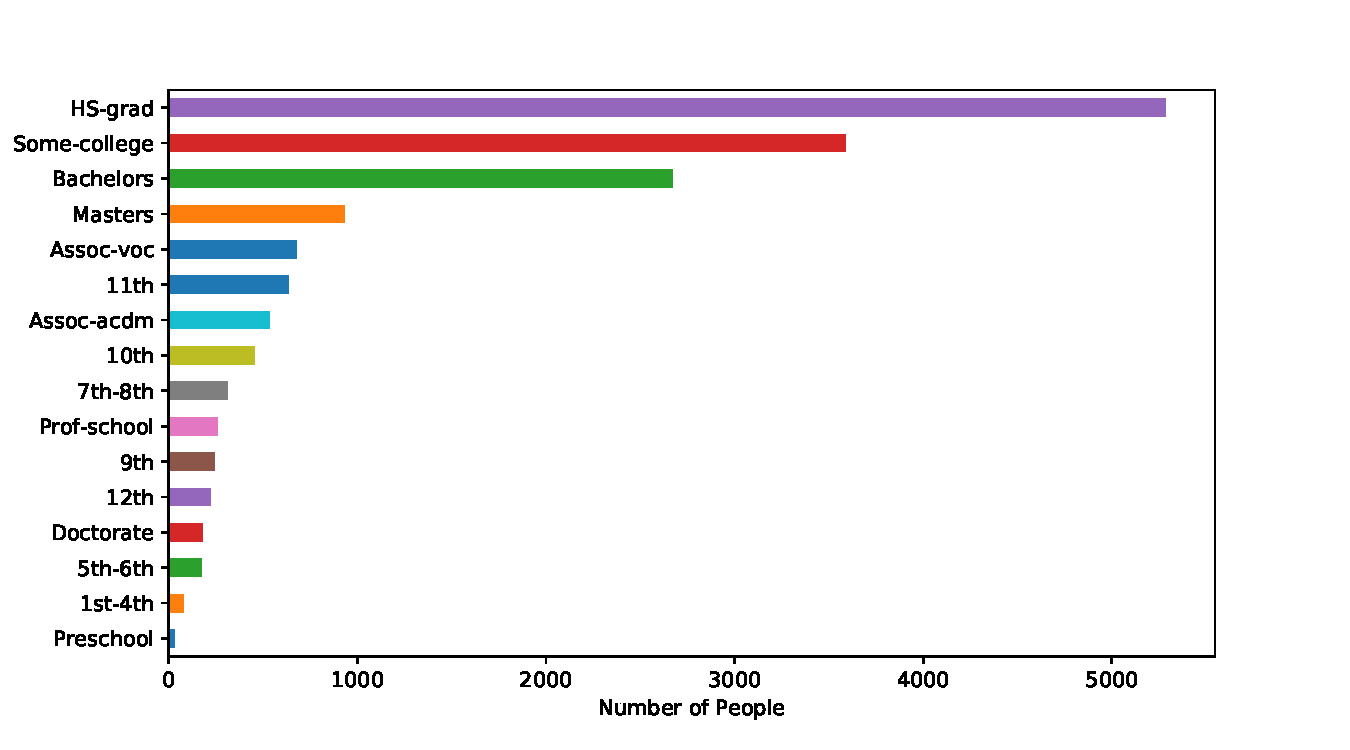
\includegraphics[width=0.48\linewidth, height=0.35\linewidth]{img/education_dis.pdf}
	}	
	\subfigure[Family Distribution]{
		\label{fig::family}
	    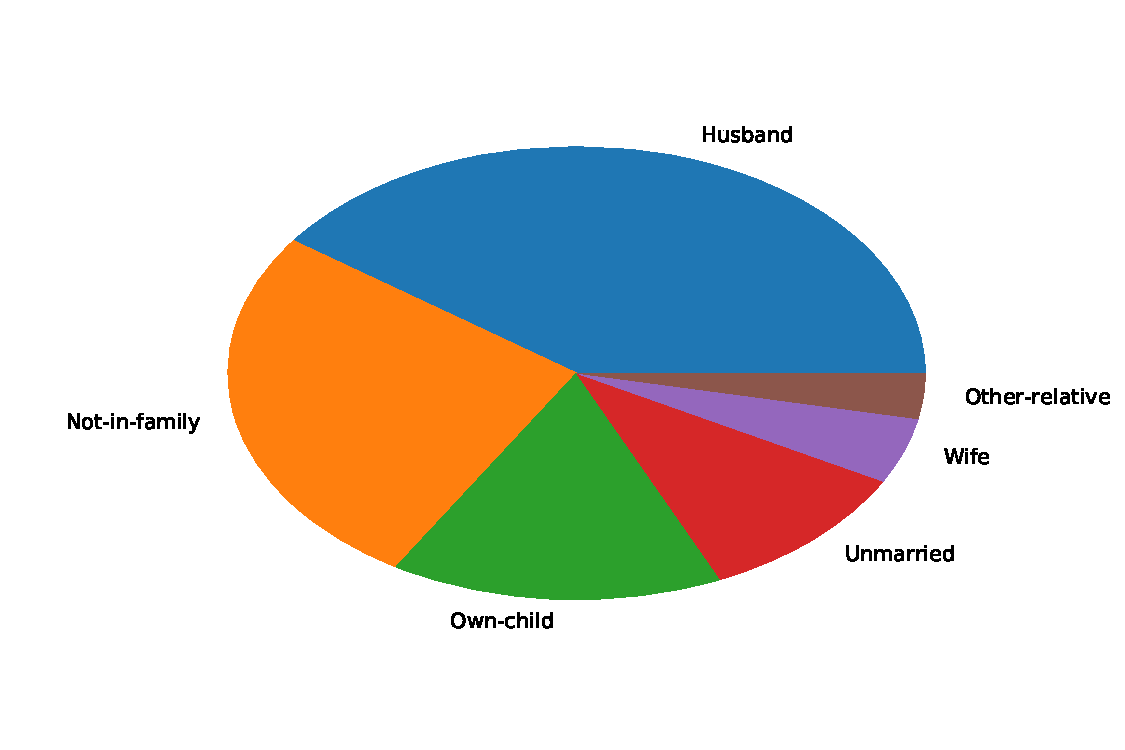
\includegraphics[width=0.44\linewidth, height=0.4\linewidth]{img/family_dis.pdf}
	}
	\subfigure[Work Time Distribution]{
		\label{fig::work_time}
		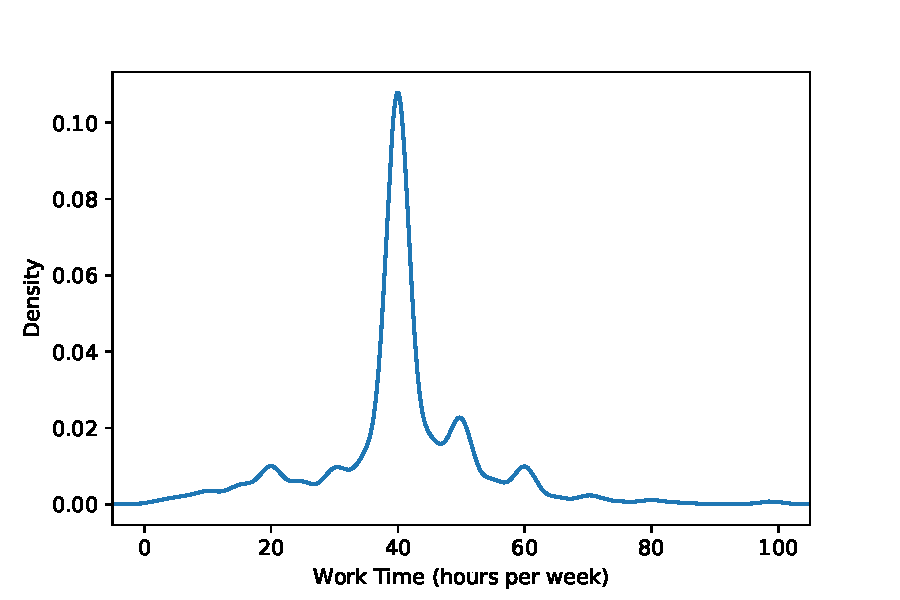
\includegraphics[width=0.6\linewidth]{img/worktime_dis.pdf}
	}
	\caption{The Distribution of Some Single Attributes.}
	\label{fig:"single_dis}
\end{figure}

\subsection{The Relation between Two Attributes}
\label{sec::relation}
Generally speaking, it is not enough to extract only the distribution of single attribute. Therefore, in this section, I would explore some relations between two attributes.

\subsubsection{Salary v.s. Educational Background}
\label{sec::salary_vs_edu}
I tend to start with the relation between salary and educational backgound. The salary in \textit{Adult} dataset is divided into two catagories: \textit{more than 50K} and \textit{less or equal to 50K}. The following two bar figures (Fig. \ref{fig::single_salary}) represent the distribution of educational background under different salary.

\begin{figure}[H]
	\centering
	\subfigure[Salary is less or equal to 50K]{
		\label{fig::salary_1}
	    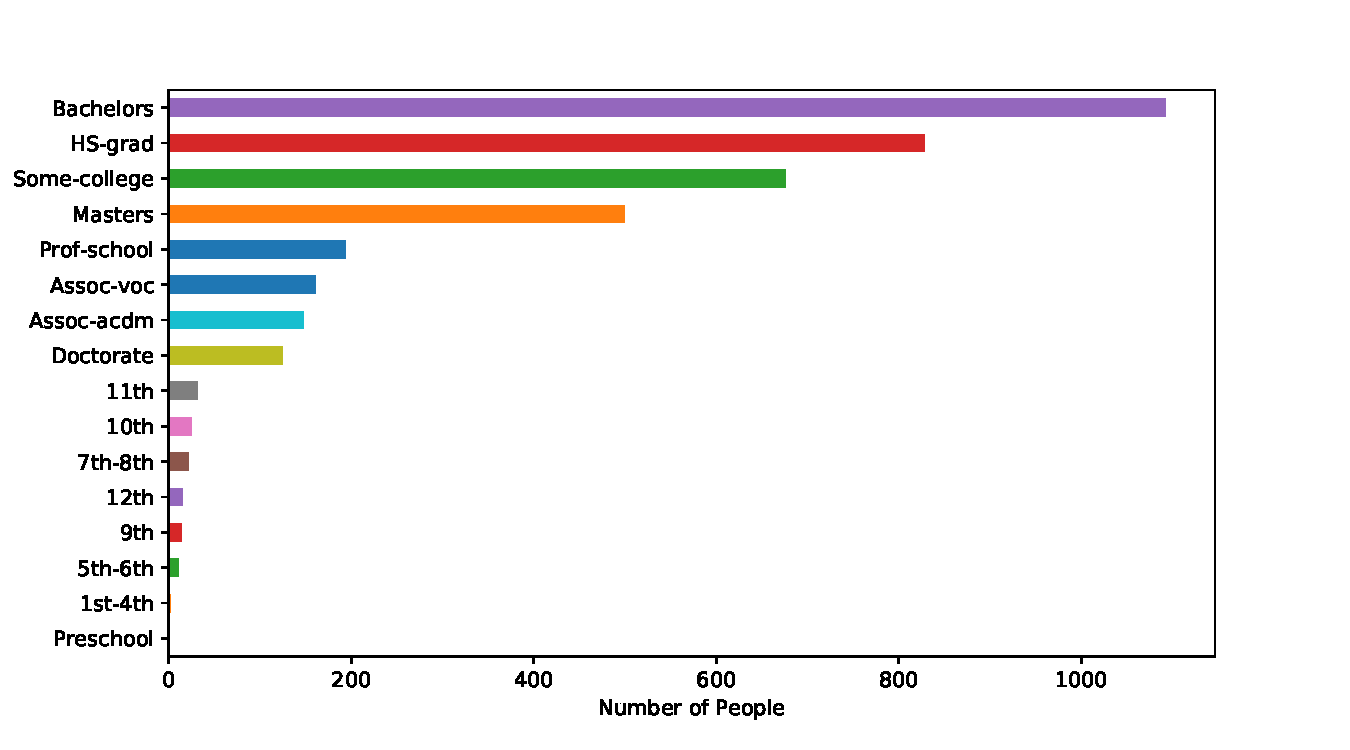
\includegraphics[width=0.483\linewidth, height=0.35\linewidth]{img/education_dis_less50k.pdf}
	}	
	\subfigure[Salary is more than 50K]{
		\label{fig::salary_2}
	    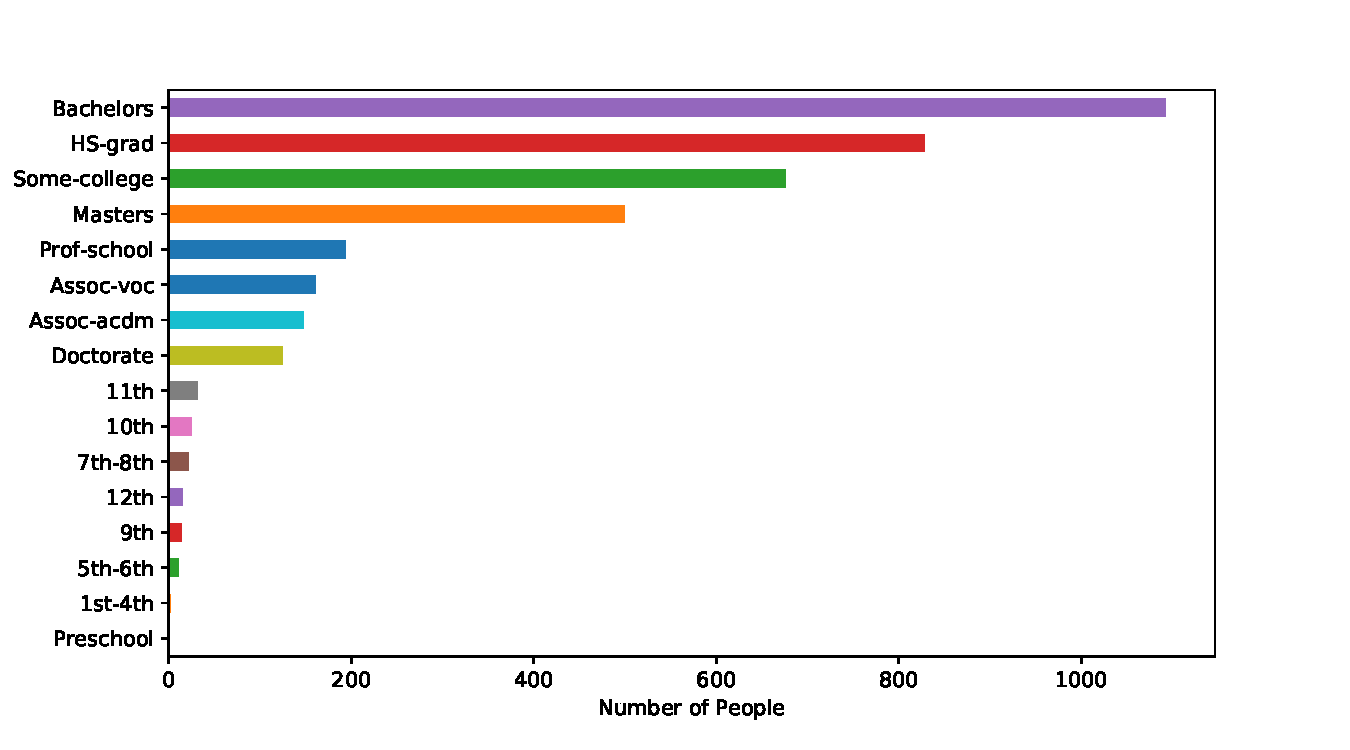
\includegraphics[width=0.483\linewidth, height=0.35\linewidth]{img/education_dis_more50k.pdf}
	}
	\caption{The distribution of educational background under different salaries.}
	\label{fig::single_salary}
\end{figure}

One of the main points implied in the two distribution is that higher education brings higher salary, which conforms to common sense.

\subsubsection{Work Time v.s. Educational Background}

I also compare the work time per week among three degrees: HS-grad, bachelor and master. (Fig. \ref{fig::worktime_vs})

\begin{figure}[H]
	\centering
	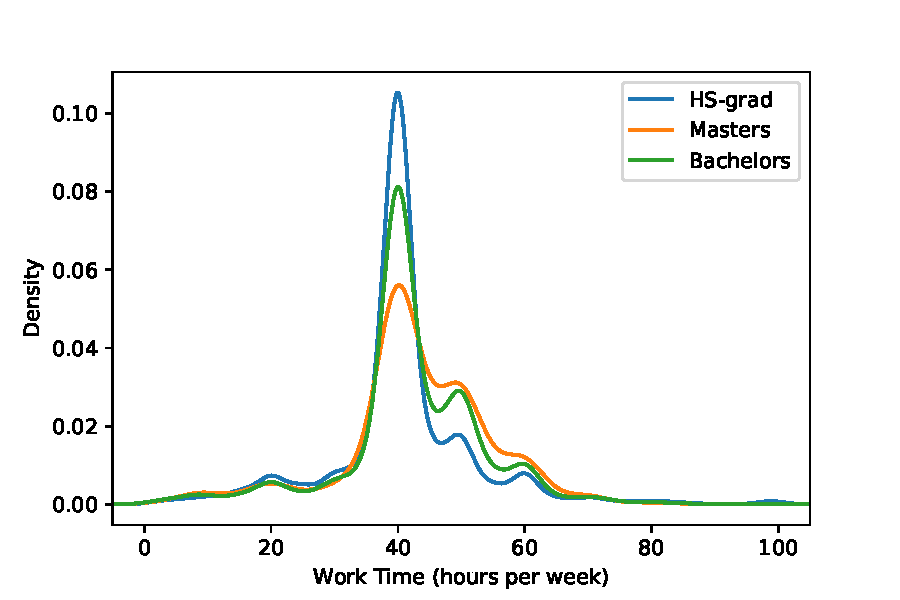
\includegraphics[width=0.75\linewidth]{img/work_time_com1.pdf}
	\caption{The work time per week among different degrees.}
	\label{fig::worktime_vs}
\end{figure}

As is shown in Fig. \ref{fig::worktime_vs}, people with a higher degree tend to invest more time in their work.

\subsubsection{Job Catagories v.s. Work Time}

I am curious about the jobs that take people more than 50 hours a week. Therefore, I plot the distribution of such jobs (Fig. \ref{fig::job}).

\begin{figure}[H]
	\centering
	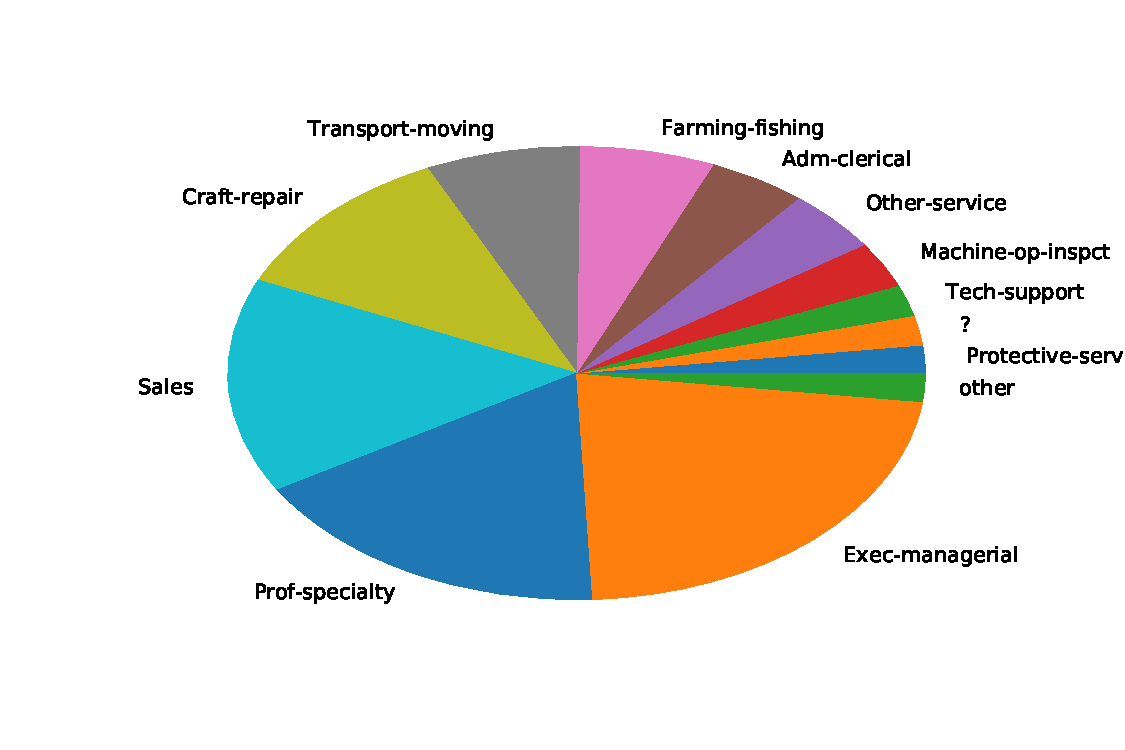
\includegraphics[width=0.75\linewidth]{img/job_dis.pdf}
	\caption{The job catagories that take people more than 50 hours a week.}
	\label{fig::job}
\end{figure}

Different from my intuition, the result indicates that time-consuming jobs are focused on management and research fields, instead of manufacturing industry.

\section{Conclusion and Discussion}
In this project, I carry out the visualization and exploration of \textit{Adult} dataset and discover some interesting phenomenons reflected from it.

According to the results of above analysis, the distribution of each attribute has some kinds of relation with others. Thus, I think I can train a model to decode this relation as some weights and predict target attributes from others in my future learning process.

Ultimately, I tend to express my sincere thanks to Professor Chaojun Lu for his patient explanation and guidance in lectures! Thank you!
{\small

\renewcommand{\refname}{References}
\bibliographystyle{ieeetr}
\bibliography{bio}
%========================================================================
\end{document}